%!TEX root = ./main.tex
%
% This file is part of the i10 thesis template developed and used by the
% Media Computing Group at RWTH Aachen University.
% The current version of this template can be obtained at
% <http://www.media.informatik.rwth-aachen.de/karrer.html>.

\chapter{Hardware Prototype and Software }
\label{ownwork} 


In this chapter we present the construction of the hardware setup and the user study software. 
Furthermore we talk about the technical considerations regarding each component and their feasibility.


\section{System Design}
The aim of this thesis is to investigate the perception of several feedback modalities underwater and their feasibility for low level navigation cues.
We include visual, auditory, and tactile feedback in form of a LED, waterproof in ear headphones,  a vibration motor, and a thermoelectric cooling module.
The prototype has to incorporate these methods as unobtrusive and comfortable as possible in particular when they are  inactive. 
Electronic connections have to be waterproof, undisturbing, and failsafe.
Furthermore all components should be affordable to provide an advantage over commercial solutions.

To investigate the recognition times and comfort of each technique we built a prototype composed of one LED in the diving goggles as well as a waterproof vibration motor and a peltier cooling module in a stretchable headband.
The headphones are provided separately.

\paragraph{Visual Feedback}

To provide visual low level feedback we use a common red 5mm LED.
An issue regarding luminous light emitted by an LED is its proneness to water reflections.
These reflections change rapidly due to water undulation and exterior lighting.
The color of the surroundings influence it as well.
For example light blue tiles in a swimming pool render a blue LED almost undetectable.
To provide clear recognizable feedback we tested several colors underwater and came to the conclusion that red LED is better recognizable than other common LED colors.

There are several ways to provide feedback with an LED.
Depending on the way it is presented the user might not notice it fast enough if the brightness increases over time.
However, this might be more comfortable than turning on the LED to full brightness instantly.
Therefore we implement both.
First we set the bright from to full brightness immediately.
Second we increase the brightness from 0\% to 100\%  and back to 0\% over 5.1 seconds resulting in a slowly blinking pattern.
We choose this interval arbitrarily after testing several durations.
This can be further investigated but would go beyond the scope of this thesis since we aim to consider several modalities.


\paragraph{Auditory Feedback}

For auditory feedback we choose AGPTEK E11B IPX8 waterproof in-ear headphones.
The headphones are worn separately from the other components and are connected to the operating MacBook Pro.
Like visual feedback, the comfortability of auditory feedback depends on the way it is presented to the user. 
The audio file played should start immediately and be clearly recognizable.
Furthermore the pitch and loudness should be within an appropriate range.
We use the sound of a sonar since it suits the underwater scenario.


\paragraph{Vibration Feedback}

To provide feedback using vibration actuators we choose waterproof 7mm vibration motors.
They are working at 3.3V with 2.45g at 250Hz.
We tried to make smaller vibration motors waterproof.
Using shrinking tubing and epoxy resin adhesive made them waterproof but running them over night underwater let them stop working regardless.
Thus we have to stick to the larger motor.

We handle the vibration feedback similar to the visual feedback and set it to maximum power instantaneously as well as increasing it over time.
Test have shown that it requires a certain amount of voltage to feel a vibration even outside the water.
Therefore we start at 1,18V and increase to 3.3V over 5.4 seconds.


\paragraph{Thermal Feedback}

For thermal feedback we choose a CUI CP6014 Thermoelectric Module. 
\cite{Peiris_thermoVR} have shown that users prefer cooling over heating.
Cooling also performs better when it comes to recognition time.
Previously we tested heating and cooling effects in water with 21 degrees and cooling was much faster perceivable than heating.
Additionally heating effects were rarely recognizable.
The peltier module has a maximum voltage of 2.1V and maximum current of 6A.
Therefore we use an external battery combined with a relay to run it.
There are specific circuit boards to control the temperature of thermoelectric cooing elements.
However we considered that running it on full power is sufficient for our purpose since we are interested in the fastest possible reaction times underwater.


\subsection{Hardware Prototype}
\todo{more pictures of prototype creation and the electronics}

As shown in figure \ref{fig:ledcloseup} the LED is glued to the diving goggles.


\begin{figure}
	\includegraphics[width= \textwidth]{images/LEDcloseupcut.png}
	\caption{LED insulated and attached between the silicone and frame of the diving goggles using hotglue. }~\label{fig:ledcloseup}
\end{figure}


Figure~\ref{fig:studysetupcut} shows the prototype parts worn by the user.
 
\begin{figure}
	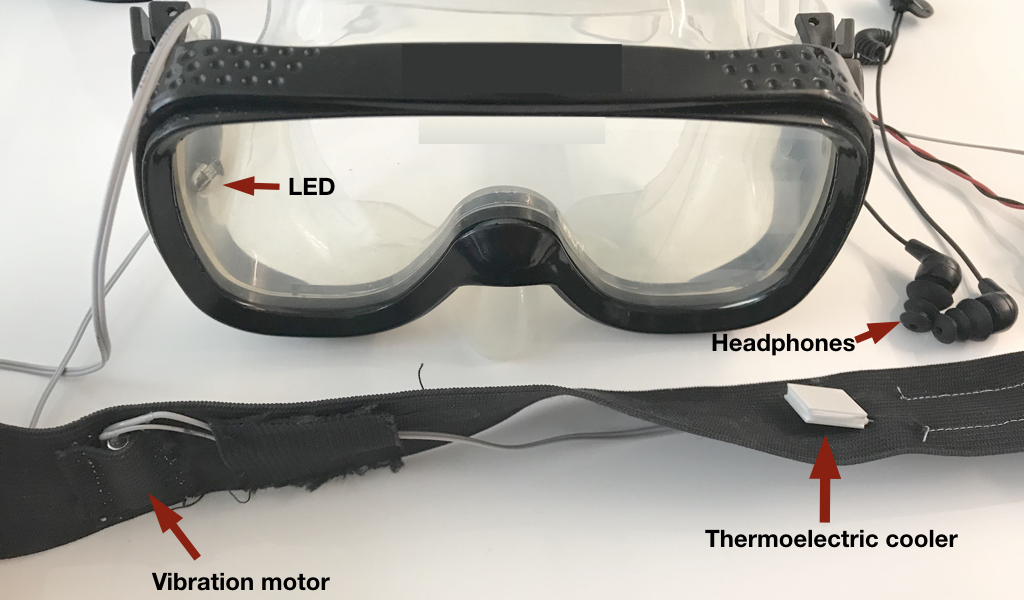
\includegraphics[width= \textwidth]{images/studysetupcut.png}
	\caption{Headband, diving goggles, and waterproof headphones with the integrated LED, Vibration motor, and Thermoelectric cooling module.}~\label{fig:studysetupcut}
\end{figure}

\begin{figure}
	\includegraphics[width= \textwidth]{images/breadboard.png}
	\caption{The Arduino controlling the relay and other components of the prototype via the ribbon cable. The batteries power the peltier when the relay is set correspondingly.}~\label{fig:ledcloseup}
\end{figure}

\begin{figure}
	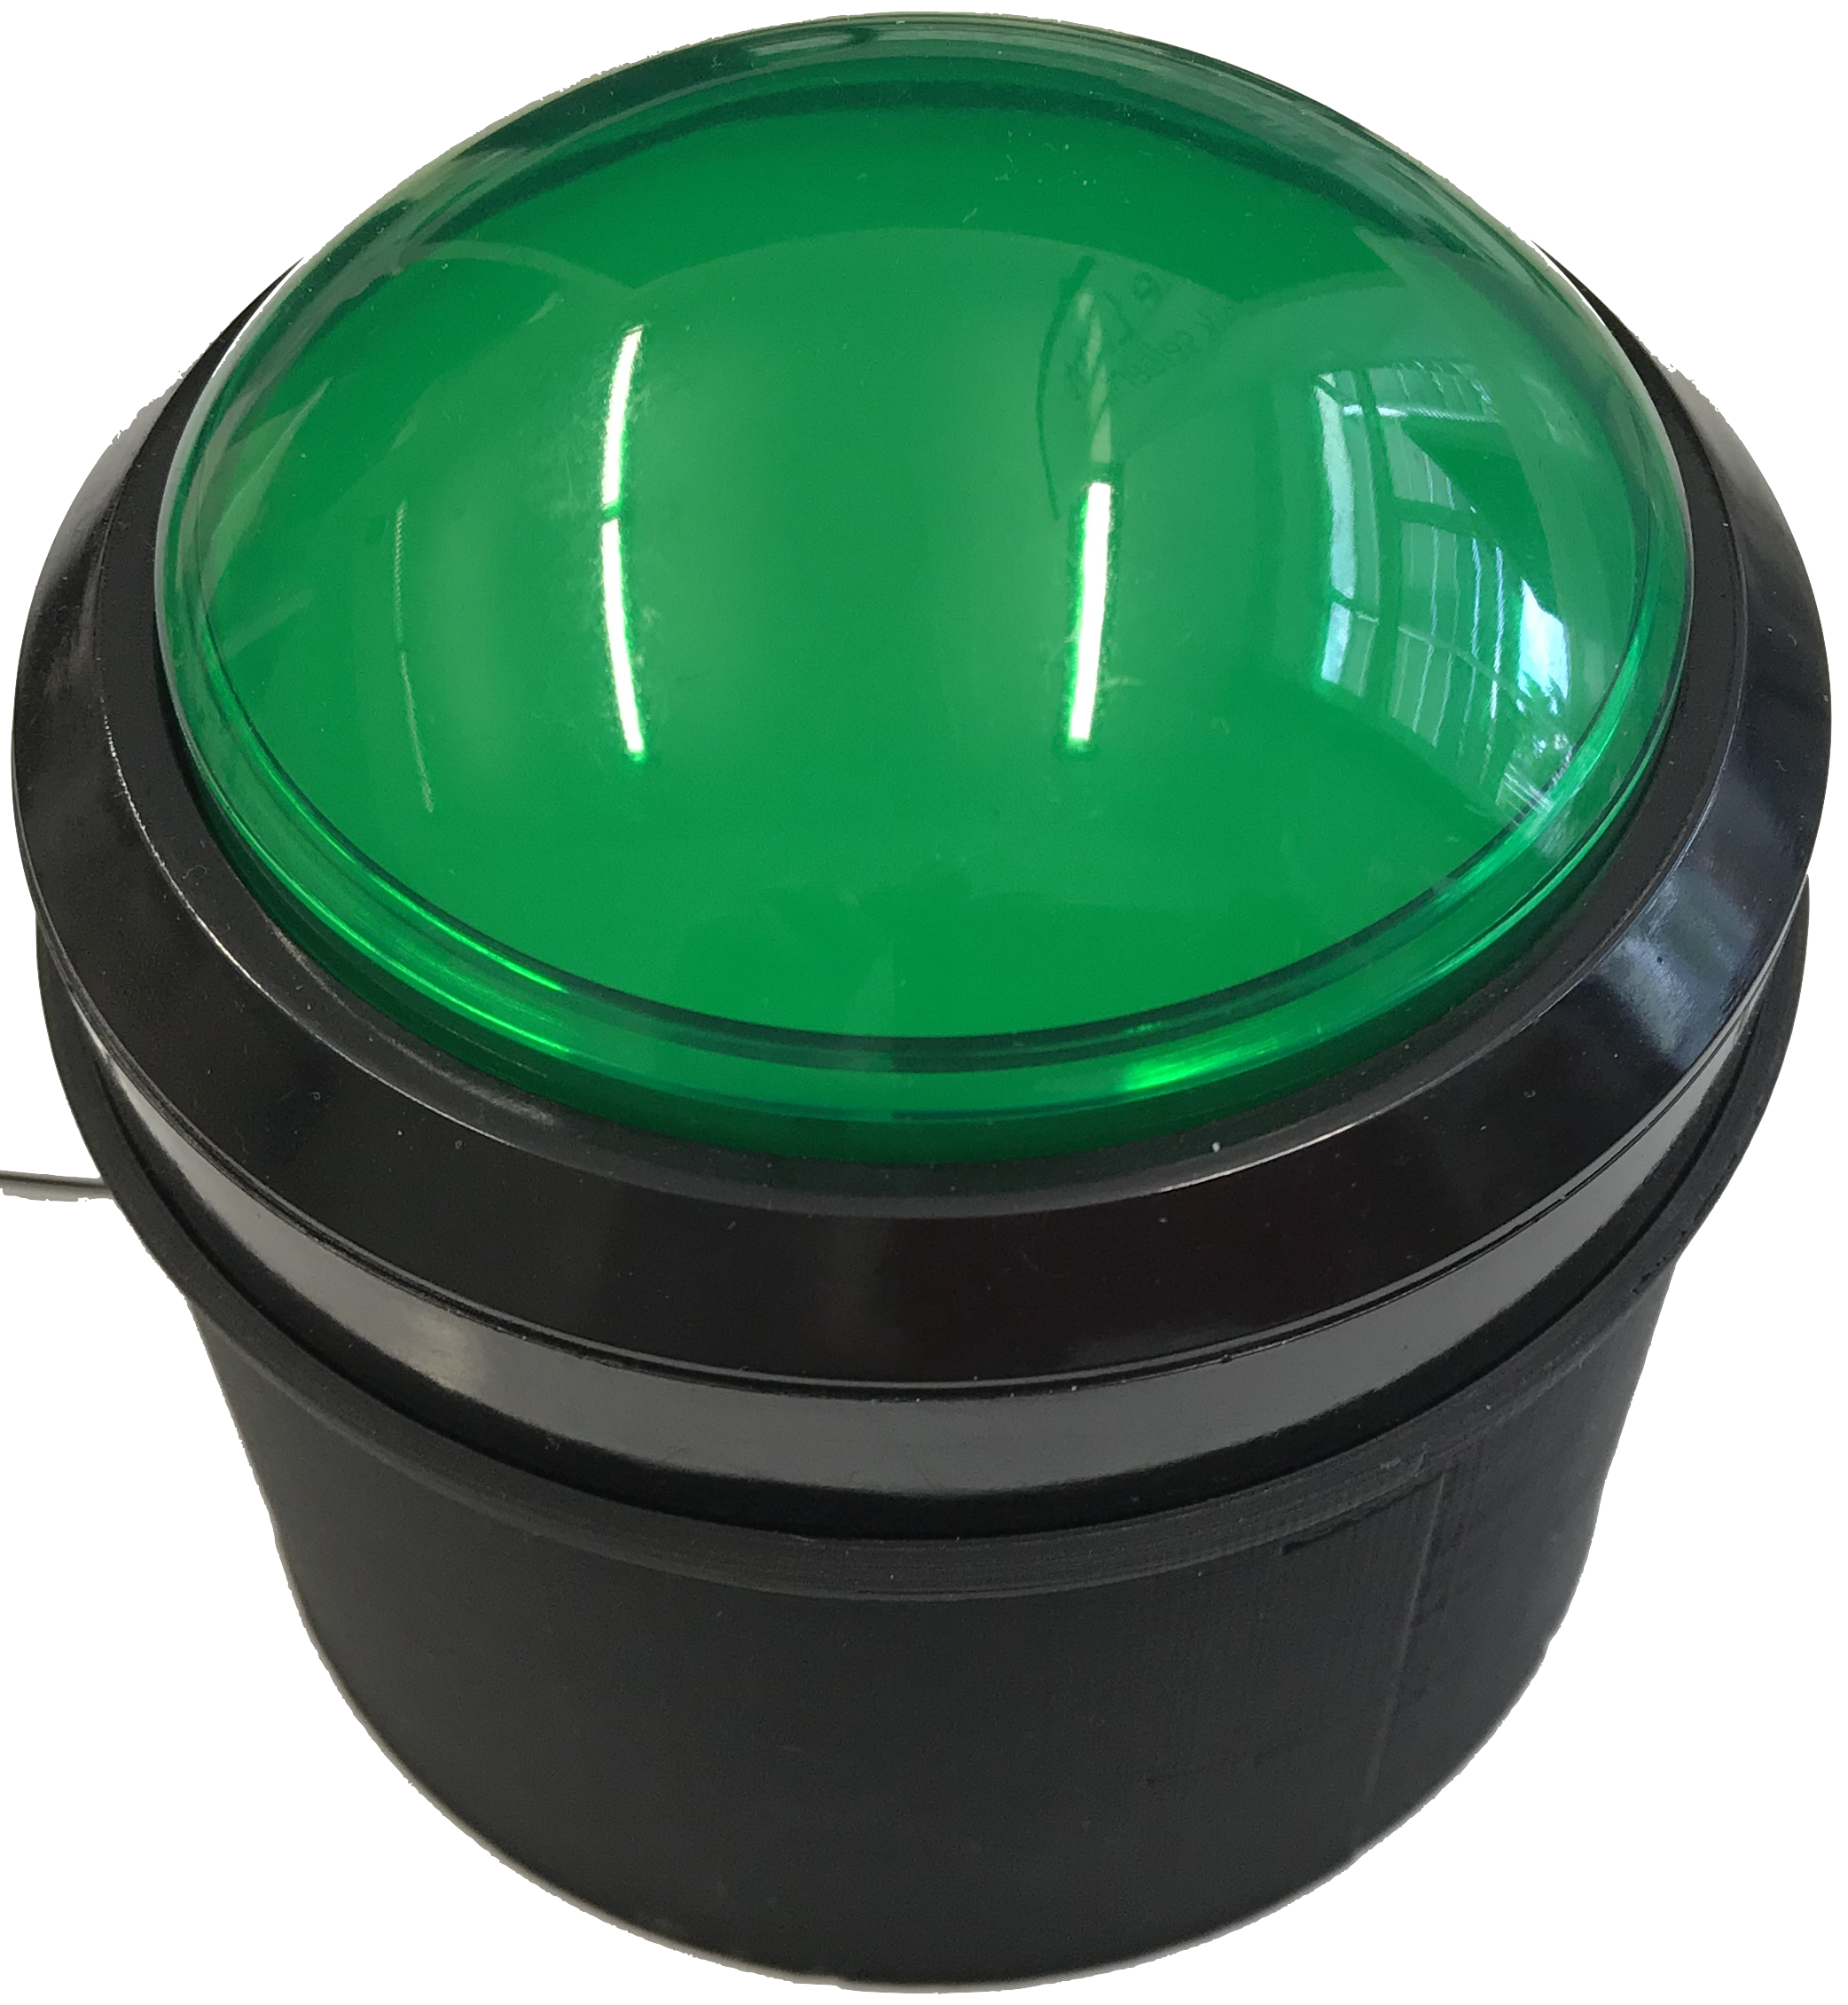
\includegraphics[width= \textwidth]{images/button.png}
	\caption{The botton and the 3D printed case. To be pressed by the user when he recognizes feedback.}~\label{fig:ledcloseup}
\end{figure}


\subsection{Testing}


 
\subsection{Safety}




\section{Software}
